\documentclass[conference]{IEEEtran}
\IEEEoverridecommandlockouts
\usepackage{cite}
\usepackage{amsmath,amssymb,amsfonts}
\usepackage{graphicx}
\usepackage{textcomp}
\usepackage{xcolor}
\usepackage{booktabs}

% ---------------------------------------------------------------
% FLAG / PLACEHOLDER: anything still needing a live check or a
% decision from Josie before July 31. Renders in red so it cannot
% be missed in the compiled PDF. Search \FLAG and \PLACEHOLDER
% before final submission and delete every one.
% ---------------------------------------------------------------
\newcommand{\FLAG}[1]{\textcolor{red}{[FLAG: #1]}}
\newcommand{\PLACEHOLDER}[1]{\textcolor{red}{[PLACEHOLDER: #1]}}

\begin{document}

\title{Can It Ford? Query-Conditioned, Physically Viable World Models for\\
Autonomous-Vehicle Flood Traversability from Gaussian Splatting
\thanks{This work was supported by the National Science Foundation under NSF REU Site: Cyberinfrastructure Research for Societal Advancement (SCIPE-AI), Award \#2447887.}}

\author{
\IEEEauthorblockN{Josie Cerrell}
\IEEEauthorblockA{
Kravis Department of Integrated Sciences \\
Claremont McKenna College \\
SCIPE-AI Research Experience for Undergraduates \\
Texas Advanced Computing Center, The University of Texas at Austin \\
jcerrell29@cmc.edu
}
}

\maketitle

% =================================================================
% ABSTRACT
% Locked, Kumar-approved, June 18 (CanItFord_Abstract_FINAL.docx).
% Reflowed into one continuous paragraph, no internal bold labels,
% since IEEE abstracts do not use run-in headers. No wording
% changed beyond removing the Background/Objective/etc. labels.
% =================================================================
\begin{abstract}
Flooded roads are a leading cause of vehicle fatalities each year, killing drivers who cannot judge how deep the water is, how fast it moves, or what the road beneath it is doing. Neither human drivers nor automated vehicles can read these things from appearance alone. World models that predict only appearance inherit the same limitation, since they can render an outcome that looks plausible but is physically wrong. This motivates physically viable world models, which preserve the latent physics that actually governs what happens when a vehicle enters floodwater. This project asks a deliberately narrow question: can an autonomous vehicle ford a specific flooded road? It then identifies the simplest physical abstraction sufficient to answer that query reliably, rather than the most detailed simulation that can be built. We reconstruct a flooded-road scene using 3D Gaussian splatting (gsplat). Following PhysGaussian, the Gaussian kernels seed a continuum representation that initializes a Material Point Method (MPM) simulation in the Genesis physics engine, where rigid-MPM coupling allows a rigid vehicle to interact with weakly compressible floodwater. We compare three levels of physical fidelity: a static depth threshold, a depth-velocity stability criterion, and, where it can be stabilized within the project timeline, a full coupled MPM simulation. Where feasible, we expect the coupled model to reproduce empirical instability thresholds, with buoyancy near published float depths and sliding governed by the depth-velocity product. Our central claim is that the minimal sufficient abstraction is query-dependent: a simple threshold suffices for deep, still water, while fast, shallow flow requires the coupled model to return the correct answer. This work delivers a reconstruct-to-decide pipeline and a concrete instantiation of query-conditioned, physically viable world models, and a small, testable step toward autonomous systems that can physically reason about a hazard before committing to it.
\end{abstract}

\begin{IEEEkeywords}
physically viable world models, Gaussian splatting, Material Point Method, flood traversability, autonomous vehicles, abstraction selection
\end{IEEEkeywords}

% =================================================================
% I. INTRODUCTION
% =================================================================
\section{Introduction}

Flooded roads kill more people in the United States each year than any other flood-related hazard, and most of those deaths involve a vehicle driven into water whose depth, flow velocity, or submerged road condition could not be judged from the surface \cite{nws_tadd}. This is not only a human-driver problem. An autonomous vehicle facing the same scene has the same information gap, and a world model that predicts only visual appearance can render a plausible-looking outcome that is physically wrong: it may show a vehicle continuing forward with no indication that the same maneuver would cause loss of traction or flotation.

Physically viable world models (PVWM) address this by preserving the latent physics that governs an action's outcome rather than only its appearance \cite{thorpe2026pvwm}. The PVWM framework identifies automatic abstraction selection, choosing how much physical fidelity a given query actually requires, as a central open problem, and leaves the orchestrator that would make that choice unimplemented \cite{thorpe2026pvwm}.

This project instantiates that orchestrator for one deliberately narrow query: \emph{can this specific autonomous vehicle ford this specific flooded road right now?} Rather than building the highest-fidelity simulation possible, we identify the simplest physical abstraction sufficient to answer that query correctly, and characterize where a cheaper abstraction silently gives the wrong answer. Figure~\ref{fig:pipeline} summarizes the full reconstruct-to-decide pipeline. The Gaussian splatting front end reached structure-from-motion on one real scene but was not trained or coupled to any result reported here, so the flood domain in every result below is specified parametrically in depth and velocity rather than recovered from reconstruction.

\begin{figure*}[t]
\centering

\includegraphics[width=0.92\textwidth]{pipeline_diagram_v2.pdf}
\caption{The reconstruct-to-decide pipeline: a real video is reconstructed as a Gaussian splat, bridged to Material Point Method particles following PhysGaussian, simulated with rigid-fluid coupling, and resolved to a FORD/NO-FORD verdict by the L0/L1/L2 abstraction orchestrator. Dashed stages are conceptual, not the path used for any result reported here: the Gaussian-splat reconstruction and the PhysGaussian kernel-to-particle bridge are designed and not yet built. The MPM stage names the solver that produced the coupled runs reported in Section~\ref{subsec:sweep}; Genesis is the engine the full pipeline is designed around.}
\label{fig:pipeline}
\end{figure*}

% =================================================================
% II. PRIOR WORK
% =================================================================
\section{Prior Work}
\label{sec:prior}

\subsection{Flood-Vehicle Stability Criteria}
Two families of empirical criteria describe when floodwater destabilizes a vehicle. The Australian Rainfall and Runoff (AR\&R) Project 10 guidelines define a depth-velocity hazard scalar, $H = D \times V$ (m\textsuperscript{2}/s), with published class-specific thresholds \cite{shand2011arr}. Those thresholds are labelled ``draft interim'' by the report itself, so throughout this paper L1 is treated as a documented decision rule to be tested rather than as a validated safety boundary. Smith, Modra, and Felder measured full-scale flotation and sliding stability curves by testing real vehicles rather than scale models \cite{smithmodrafelder2019}. Their small passenger car was a Toyota Yaris sedan, tested at full scale alongside a Nissan Patrol 4WD and a Ford Festiva, and it is the same vehicle model this paper simulates at L2 \cite{smithmodrafelder2019}. Both are single-number criteria: neither represents the direction of applied force, and neither was derived to predict the persistent lateral drift this project observes at some phase-space points (Section~\ref{sec:results}).

\subsection{Physics-Grounded Scene Reconstruction}
3D Gaussian Splatting (3DGS) reconstructs a photorealistic, explicit scene representation from ordinary multi-view video \cite{kerbl20233dgs}. PhysGaussian extends this representation with physical simulation by treating each Gaussian kernel's covariance as a seed for a continuum Material Point Method (MPM) particle volume, allowing a trained splat to drive a physics simulation directly rather than only a renderer \cite{xie2023physgaussian}. The simulation itself runs in Genesis, an open-source, solver-agnostic physics engine \cite{genesis2024}. We are not aware of a publicly available, drop-in pipeline carrying flood video through to a Genesis MPM simulation: PhysGaussian's own reference implementation targets a Warp MPM solver rather than Genesis, so the bridge between the two is built here rather than adopted.

\subsection{Why a Single Scalar Threshold Is Insufficient}
Both L0 and L1 are deterministic functions of published thresholds, not simulation output: L0 applies a single fixed depth cutoff \cite{nws_tadd}, and L1 applies the AR\&R two-part depth-and-hazard criterion per vehicle class \cite{shand2011arr}. We evaluate both across the same depth-velocity grid. Fig.~\ref{fig:l0l1} shows that L0 alone is markedly over-conservative, and that AR\&R's own published per-class caps (Fig.~\ref{fig:threeclass}) already diverge well before any coupled simulation is involved. Neither figure required simulated data; both are direct evaluations of cited formulas, and both motivate why a coupled physical model is worth the added cost.

\begin{figure}[t]
\centering
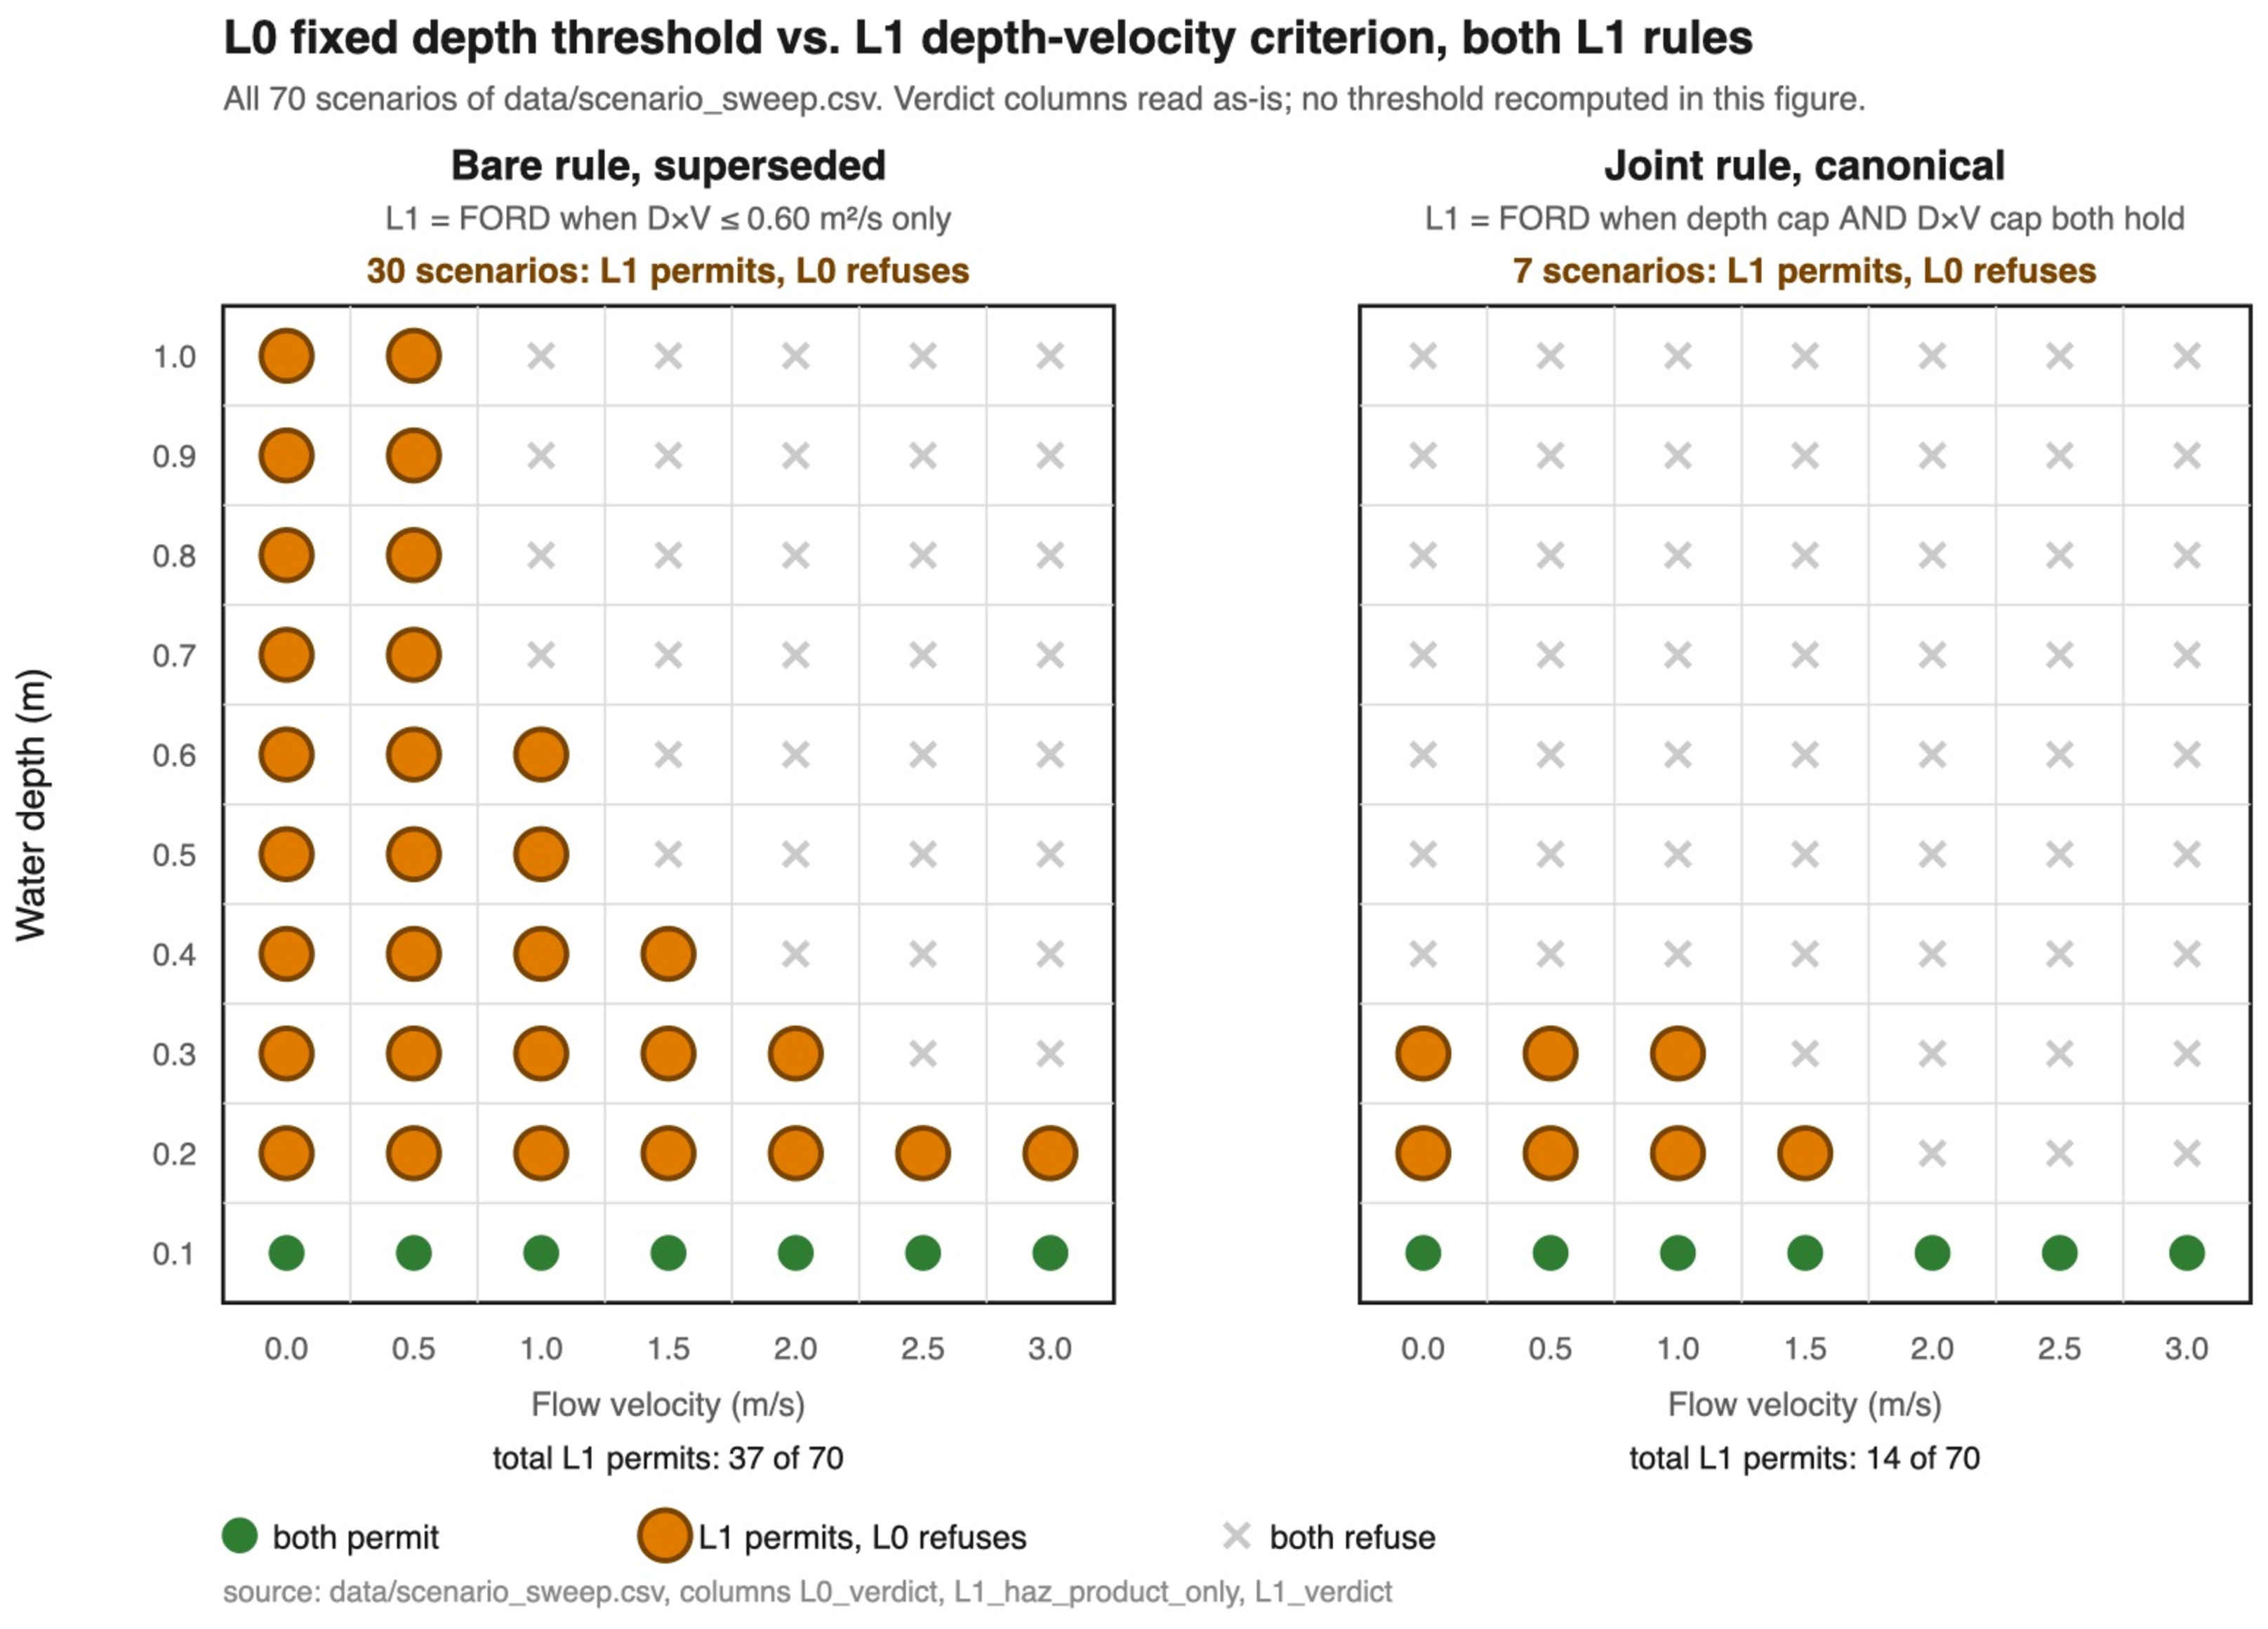
\includegraphics[width=\linewidth]{l0l1_two_rules_v2.pdf}
\caption{L0 (fixed depth threshold) versus L1 (AR\&R depth-velocity criterion) across all 70 (depth, velocity) scenarios of \texttt{data/scenario\_sweep.csv}. Both panels are direct evaluations of published formulas \cite{nws_tadd,shand2011arr}, not simulation output, and both read their verdicts from stored columns rather than recomputing a threshold. Left: the \emph{bare} rule (\texttt{L1\_haz\_product\_only}), which tests only $D \times V \le 0.60$\,m\textsuperscript{2}/s and permits crossing in 37 of 70 scenarios, 30 of them where L0 alone would refuse. Right: the \emph{joint} rule (\texttt{L1\_verdict}), which requires the class depth cap, the 3.0\,m/s velocity cap, and the $D \times V$ cap to all hold together, permitting 14 of 70, only 7 of them beyond L0. The joint rule is canonical for this paper going forward; the bare rule is shown because it is the form in which the criterion is most often applied. The two panels differ in both rule structure and vehicle class: the left applies AR\&R's Large 4WD hazard cap alone ($D \times V \le 0.60$\,m\textsuperscript{2}/s, no depth restriction), the right the Small Car joint rule ($D \times V \le 0.30$\,m\textsuperscript{2}/s \emph{and} depth $\le 0.30$\,m); \texttt{L1\_verdict} is identical to \texttt{L1\_verdict\_small\_passenger} on all 70 rows. Of the 23 scenarios that reclassify from FORD to NO-FORD between the panels, 5 are excluded by the tighter hazard cap alone, 10 by the depth cap alone, and 8 by both, and none reclassify in the opposite direction. The depth cap is not redundant with the hazard cap: 7 of the 23 are standing water at zero velocity and depths of 0.40 to 1.00\,m, which a product-only threshold permits at any depth because $D \times V = 0$.}
\label{fig:l0l1}
\end{figure}

\begin{figure}[t]
\centering
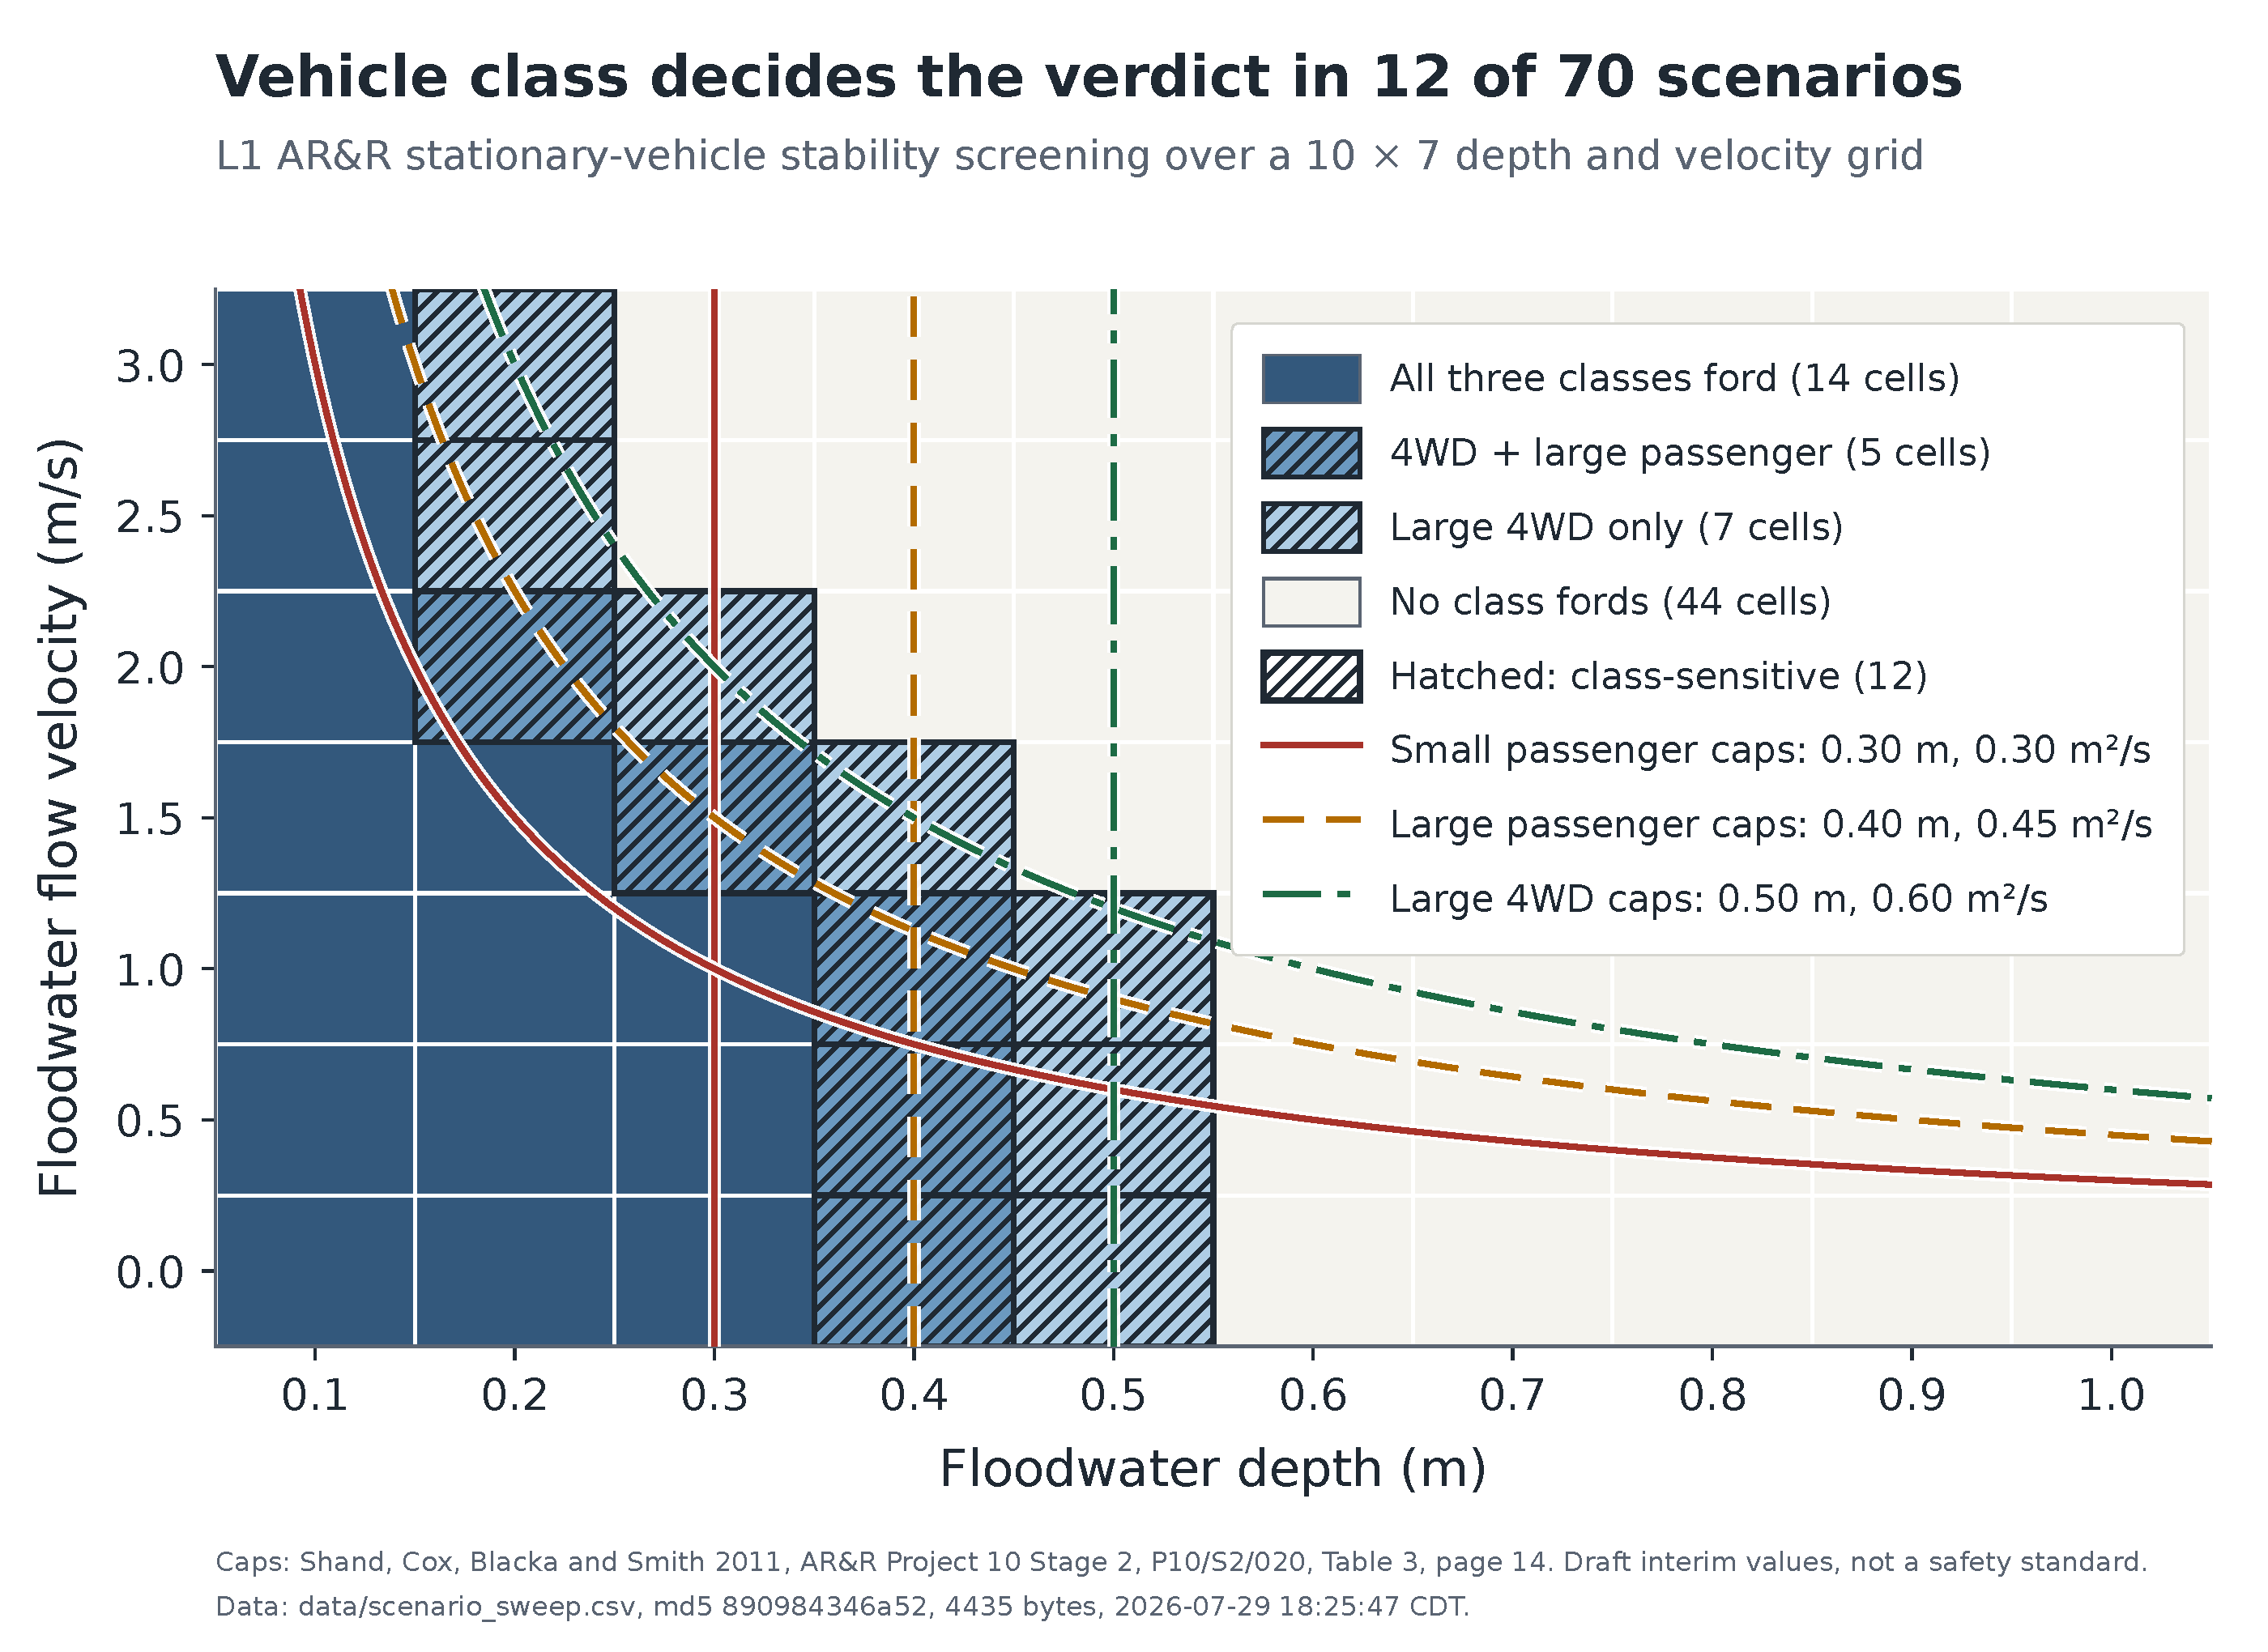
\includegraphics[width=\linewidth]{L1_three_class_corrected.pdf}
\caption{The L1 criterion evaluated per AR\&R's own three published vehicle classes \cite{shand2011arr}: small passenger, large passenger, and large 4WD. These do not correspond to the sedan/SUV/pickup grouping used for the diagnostic vehicle asset in Table~\ref{tab:vehicle}. That grouping is ours: it is assembled from individual measured vehicle inertial parameters \cite{heydinger1999sae}, not from any published three-class scheme. Where this paper reports results tied to AR\&R's own classes, it uses the watertight-hull mass-override method described in Section~\ref{sec:approach}-C, not the silhouette splat.}
\label{fig:threeclass}
\end{figure}

\subsection{Forward and Inverse Property Estimation}
Hsiao and Kumar demonstrate the inverse direction of this same reconstruction-to-physics pipeline: given only visual observation, a NeRF-based reconstruction paired with Bayesian optimization recovers a granular material's friction angle to within roughly two degrees of ground truth \cite{hsiao2025nerfmpm}. This project addresses the complementary forward direction: given a known scene and known flood hydraulic conditions, what is the traversability verdict under full fluid-rigid-body dynamics? Together, the two directions describe a closed perception-to-action loop, one of the auditability properties PVWM requires \cite{thorpe2026pvwm}.

% =================================================================
% III. APPROACH
% =================================================================
\section{Approach}
\label{sec:approach}

\subsection{Pipeline}
The reconstruct-to-decide pipeline (Fig.~\ref{fig:pipeline}) has four stages: (1) a real flooded or water-adjacent road scene is captured on video and reconstructed in 3D via Gaussian splatting on an NVIDIA A100 GPU (TACC Lonestar6); (2) following the PhysGaussian extraction pattern, trained Gaussian kernels are opacity-filtered and converted into an initial MPM particle volume; (3) the particle volume, together with a rigid-body vehicle proxy, is simulated with weakly-compressible MPM water and rigid-MPM coupling, in the Genesis physics engine as designed and, for the coupled runs reported here, in a Warp-based MPM solver; (4) the simulation's displacement output is passed through a query-conditioned abstraction-selection orchestrator, \texttt{orchestrate\_ford\_query()}, which returns a FORD/NO-FORD verdict at the cheapest level of fidelity sufficient to answer correctly.

\subsection{Three-Level Abstraction Ladder}
We compare three levels of physical fidelity on the same phase-space grid of (depth, velocity) conditions, summarized in Table~\ref{tab:ladder}.

\begin{table}[t]
\caption{Abstraction Ladder Definitions}
\label{tab:ladder}
\centering
\begin{tabular}{@{}p{0.3in}p{0.55in}p{2.25in}@{}}
\toprule
\textbf{Level} & \textbf{Basis} & \textbf{Definition} \\
\midrule
L0 & Depth & Fixed depth cutoff at 0.15\,m, independent of velocity or vehicle class. This is the National Weather Service's 6-inch figure, the depth at which fast-moving water can knock over an adult; the same source's vehicle figure is twice that, 12 inches (0.30\,m), at which rushing water carries away most cars \cite{nws_tadd}. We adopt the pedestrian depth deliberately, as the conservative bound of the two, and note that full-scale testing does not give one number here. A small car can lose stability in roughly 0.15\,m of fast-moving water, while the still-water depth at which it floats is closer to 0.30\,m \cite{smithmodrafelder2019}. A single L0 cutoff is therefore standing in for two different situations, and which one it matches depends on how fast the water is moving. Across the 70-scenario grid this admits 7 scenarios; the 0.30\,m cutoff would admit 21. \\
L1 & $D\times V$ & AR\&R's joint criterion. A crossing is permitted only when all three limits hold at once: depth at or under the class cap, velocity at or under 3.0\,m/s, and $D \times V$ at or under the class product cap \cite{shand2011arr}. For small passenger those are 0.30\,m, 3.0\,m/s, and 0.30\,m\textsuperscript{2}/s. The velocity limit never binds on our grid, which stops at 3.0\,m/s. $V$ is flow velocity, not vehicle speed. Mass and force direction are not represented. \\
L2 & MPM & Coupled rigid-body/MPM simulation; NO-FORD when lateral drift exceeds 0.05\,m. That value is an internal numerical detector for onset of motion, set conservatively above the solver's own displacement noise floor, and is not itself an empirical stability criterion. The sliding physics it stands in for, drag overcoming tyre-road friction on a partially submerged vehicle, is established independently \cite{shah2018,xia2014}. \\
\bottomrule
\end{tabular}
\end{table}

This instantiates the orchestrator PVWM leaves unimplemented: the empirical L1/L2 divergence zone characterized in Section~\ref{sec:results} defines the escalation boundary at which L1 alone is not sufficient and the query must be answered at L2.

A first-principles force balance motivates why L1's scalar hazard measure is expected to be insufficient. Fig.~\ref{fig:force} plots lateral hydrodynamic drag force against maximum available static friction at several water depths (left), and the resulting critical velocity above which drag is predicted to exceed friction, as a function of depth (right). It is built from the standard quadratic drag relation, $F_D = \tfrac{1}{2}\rho C_d A V^2$, balanced against a Coulomb friction limit $\mu N$ in which the normal force $N$ is reduced by buoyancy. Both coefficients are pinned to measured primary sources. The drag coefficient $C_d = 1.38$ comes from Smith, Modra, and Felder's flume testing of a 1:18 scale Toyota Yaris, inside the 1.0 to 1.8 range they report across subcritical and supercritical flow \cite{smithmodrafelder2019}. The friction coefficient $\mu = 0.30$ is the value AR\&R itself adopted when deriving the L1 thresholds this figure interrogates, which Shand et al. call conservative \cite{shand2011arr}, and which also matches their worst-case bed friction against 0.78 for concrete; the right panel shades that band. That choice matters: the figure and the L1 criterion now rest on the same friction assumption, so divergence between them cannot be attributed to that gap. What remains unpinned is the displacement geometry, which the caption states explicitly.

\begin{figure}[t]
\centering

\includegraphics[width=\linewidth]{force_balance_v2.pdf}
\caption{Analytical force-balance calculation, not simulation output. Left: lateral drag force versus flow velocity at four depths, against the maximum static friction limit (dashed). Right: the resulting critical velocity as a function of depth, with the band spanning $\mu = 0.30$ to 0.78. Coefficients are pinned to primary sources: $C_d = 1.38$ \cite{smithmodrafelder2019}, $\mu = 0.30$ \cite{shand2011arr}, mass 1100\,kg. The legend reports $N$ directly; it is $0.00$\,kN at 0.30, 0.45, and 0.60\,m. Those zeros are a real buoyancy result, not missing values: at 0.30\,m the buoyant force reaches 16.135\,kN against a weight of 10.791\,kN, following from the effective plan area of 5.4825\,m\textsuperscript{2}, so $N$ is zero and the friction limit $\mu N$ vanishes with it. The right panel corroborates this independently, with critical velocity falling to zero at 0.201\,m. That flotation depth follows from the model's one remaining assumption, a solid prism over 0.75 of the bounding-box footprint. The hull encloses 3.5427\,m\textsuperscript{3} against a 10.7457\,m\textsuperscript{3} nominal prism (4.30 $\times$ 1.70 $\times$ 1.47\,m), a fill factor of 0.33; against the mesh's own 11.3533\,m\textsuperscript{3} extent it is 0.312. Either way the prism overstates displacement and floats the car at about 0.20\,m, shallow against the 0.34 to 0.67\,m reported for real cars and AR\&R's 0.30, 0.40, and 0.50\,m still-water limits \cite{shand2011arr}. That bias runs toward predicting loss of traction too early, and is stated here rather than absorbed into the curves.}
\label{fig:force}
\end{figure}

\subsection{Vehicle and Scene Representation}
The vehicle asset used to find and root-cause this project's grid-resolution solidification defect is a rigid body solidified from a surface Gaussian splat (\texttt{truck\_trimmed.ply}, 191{,}107 points, no interior), used because no watertight simulation-ready mesh existed in the pipeline at the time. Three vehicle classes (sedan, SUV, pickup) are each a single rescaled base silhouette stretched to bounding-box dimensions taken from individual measured vehicles in the NHTSA/SAE inertial-parameter database \cite{heydinger1999sae}. That source is a record of individually measured vehicles through November 1998; it is not a matched sedan/SUV/pickup set, and it contains no Yaris. The grouping into three classes is therefore ours, built by selecting individual entries, and carries no authority from the source beyond the per-vehicle measurements themselves. This is stated explicitly as a limitation, not glossed over: all three classes share one silhouette, so cross-class comparisons involving this asset reflect scaled mass and footprint, not distinct vehicle geometry.

Solidifying a surface point cloud into a filled rigid body is grid-resolution-dependent in a way that is easy to miss. At MPM grid resolution \texttt{n\_grid=64}, the column-fill solidification step correctly produces a solid body and the three densities in Table~\ref{tab:vehicle} are recovered. At \texttt{n\_grid=128}, the same splat produces a hollow shell instead: verified directly in job 833349 (\texttt{ford\_sweep\_driver.py --config v3}, run July 15, 2026; documented in \texttt{docs/\allowbreak track1\_v3\_\allowbreak sweep\_invalid\_\allowbreak hollow\_vehicle.md}), particle count scaled 4.31$\times$ between the two resolutions rather than the 8$\times$ a solid body requires, and 0 of 60 test runs at \texttt{n\_grid=128} passed a density plausibility check (all three classes' apparent density roughly doubled, 1.84--1.87$\times$, a resolution artifact, not a physical effect). Water resolution and vehicle solidity are governed by different length scales for this asset, raising grid resolution helps the former and silently breaks the latter. \textbf{Table~\ref{tab:vehicle}'s densities hold only at \texttt{n\_grid=64}} and must not be read across to any higher-resolution run without re-solidifying the vehicle by a decoupled method first. This also settles, rather than merely defers, the question of testing 0.05\,m depth: at \texttt{n\_grid=64} the material points sit about 0.074\,m apart, which is wider than the 0.05\,m being requested, so it seeds zero water particle layers for the pickup class, and at \texttt{n\_grid=128} the vehicle itself is invalid, so 0.05\,m is not reachable with this asset at any grid setting tested.

The candidate fix this diagnosis points to, moving to a true watertight mesh rather than re-tuning the solidification pitch, is what the project adopted for vehicle representation tied to AR\&R's own classes. A watertight 2010 Toyota Yaris hull (\texttt{yaris\_coarse\_v1l\_watertight.ply}) replaces the single rescaled silhouette with one real geometry. It comes from the crash-validated finite-element model that the Center for Collision Safety and Analysis publishes for NHTSA \cite{ccsa2016yaris}. We use 1100\,kg as the baseline mass. CCSA reports two different weights for this model: the real car they measured weighed 1078\,kg, and their finite-element version of that car weighs 1101\,kg. We simulate the mesh and not the physical car, so 1101\,kg is the figure that applies, and we round it to 1100\,kg. That also matches the 1100\,kg small-car test specification the model was built to meet. Vehicle class is then a mass override on that same geometry rather than three separate meshes (\texttt{renders/\allowbreak yaris\_render\_s1/\allowbreak gates\_both\_\allowbreak scenarios.py}): \texttt{small\_passenger} at 1100\,kg, \texttt{large\_passenger} at 1609\,kg, and \texttt{large\_4wd} at 2337\,kg. AR\&R does not publish a single mass for each class. It publishes a kerb-weight bound: under 1250\,kg for small passenger, over 1250\,kg for large passenger, and over 2000\,kg for large 4WD \cite{shand2011arr}. Each of our three masses falls inside the right bound, but they are representative values we chose, not numbers AR\&R states. This resolves the class-mapping question in Fig.~\ref{fig:threeclass}: AR\&R's classes do not map onto the sedan/SUV/pickup NHTSA/SAE classes used for the diagnostic asset in Table~\ref{tab:vehicle} at all; they are a separate three-mass study on one watertight hull, kept deliberately distinct from the silhouette-based diagnostic above. This mass-override asset and method, not the silhouette splat, is what any AR\&R-class-linked simulation result in this paper is run on. The Yaris is also the small-passenger vehicle used in the full-scale traction testing of Smith, Modra and Felder \cite{smithmodrafelder2019} and in the scale-model work of Azhar, Pauwels and Bui \cite{azhar2023}, so the simulated geometry corresponds directly to the vehicle behind the empirical stability data this work compares against.

\begin{table}[t]
\caption{Vehicle Class Density at \texttt{n\_grid=64} (Only Valid Grid Setting)}
\label{tab:vehicle}
\centering
\begin{tabular}{@{}p{0.7in}p{0.95in}p{1.1in}@{}}
\toprule
\textbf{Class} & \textbf{Density (kg/m\textsuperscript{3})} & \textbf{In heuristic band?} \\
\midrule
Sedan & 293.55 & Yes \\
Pickup & 242.12 & Yes \\
SUV & 308.13 & No (2.7\% over, left as-is) \\
\bottomrule
\end{tabular}
\\[2pt]
{\footnotesize Verified against \texttt{docs/track1\_v3\_sweep\_invalid\_hollow\_vehicle.md}. Values are not meaningful at \texttt{n\_grid=128} (see body text).}
\end{table}

% =================================================================
% IV. RESULTS
% =================================================================
\section{Results}
\label{sec:results}

\subsection{Scene Reconstruction Status}
Structure-from-motion reconstruction (COLMAP) is complete for one real scene (``Drain A''), confirmed via a populated sparse point cloud and camera pose set on TACC Vista scratch storage. Gaussian-splat training from that reconstruction runs separately on LS6 and is not complete at the time of writing, so Drain A is a finished structure-from-motion reconstruction and not yet a trained, simulation-ready splat. A second scene (``Drain B'') has not been captured or reconstructed. No result reported in this paper depends on either scene; the reconstruction stage is reported here as pipeline status, and every quantitative result below comes from synthetic geometry or the watertight hull.

\subsection{Synthetic-Geometry Pilot Study}
An early parametric comparison of L1 against a Genesis SPH solver (\texttt{data/l2\_results\_from\_wandb.csv}) covers 9 unique (depth, velocity) conditions. L1 and L2 agreed at 5 of 9 (55.6\%). The 4 divergence points, where L1 returned FORD but L2 returned NO-FORD, were (0.30\,m, 1.5\,m/s), (0.15\,m, 1.5\,m/s), (0.30\,m, 1.0\,m/s), and (0.30\,m, 2.0\,m/s). These figures supersede an earlier draft of this subsection, which reported 23 pairs, 16 divergence points, and 30.4\% agreement. Those numbers do not match this dataset and were never traced to a source file, so we treat them as unverified and report only what is read directly from the CSV. A separate file, \texttt{data/phase\_space\_results.csv}, does contain 23 unique (depth, velocity) pairs, matching the older pair count, but it carries a single verdict column with no corresponding L1 value, so no agreement rate can be computed from it; 15 of its 31 rows additionally share a condition with another row under a different verdict, with three separate (0.30\,m, 1.5\,m/s) runs returning FORD, NO-FORD, and NO-FORD at three different displacements, so it is not cleanly enough run-labelled to use as it stands. Reconciling that file against an explicit L1 calculation remains outstanding.

A separate 4-point friction sweep at the (0.30\,m, 1.5\,m/s) divergence point (\texttt{data/mu\_sweep\_results.csv}) shows lateral displacement of 0.399, 0.3957, and 0.3953\,m at coupling friction $\mu = 0.3, 0.5, 0.7$ respectively, essentially invariant across that range. At $\mu = 0.0$, displacement drops to 0.3283\,m, a real difference, not noise. The invariance therefore holds across the $\mu=0.3$ to $0.7$ range and not from zero, a distinction an earlier draft of this work elided by describing the sweep as friction-invariant across $\mu=0.0$ to $0.7$. The qualitative point is unaffected: a scalar hazard measure cannot represent this directional force. The sweep is nonetheless four points at a single condition, and we do not generalize beyond it.

Fig.~\ref{fig:l2schematic} plots that verified 9-point dataset directly. It is deliberately not extrapolated beyond those nine conditions, and the divergence structure it shows should be read as characterizing this pilot dataset rather than the full operating envelope.

\begin{figure}[t]
\centering
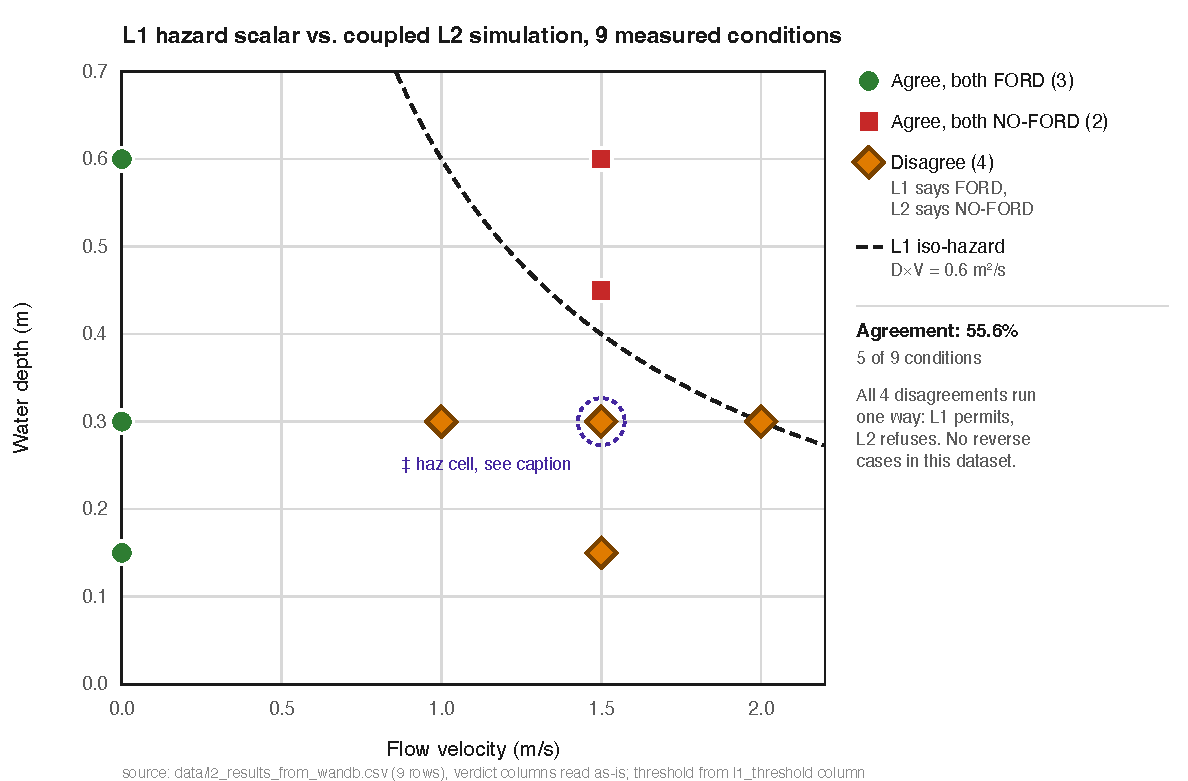
\includegraphics[width=0.85\linewidth]{l2_divergence_real_v2.pdf}
\caption{L1 hazard scalar versus coupled L2 simulation, 9 simulated conditions from \texttt{data/l2\_results\_from\_wandb.csv}. Agreement holds at 5 of 9 (55.6\%): 3 conditions where both agree FORD, 2 where both agree NO-FORD. All 4 disagreements run one way, L1 permits and L2 refuses, with no reverse cases in this dataset. One flagged cell (marked \textdaggerdbl) has an \texttt{l1\_haz\_score} that disagrees with its own $D \times V$ product; the figure plots the consistent $D \times V$ value throughout and the discrepancy is noted rather than silently resolved.}
\label{fig:l2schematic}
\end{figure}

\subsection{Real-Simulation Sweep}
\label{subsec:sweep}
These 17 runs were executed with a Warp-based MPM solver (\texttt{warpmpm}), not with Genesis; Genesis is the engine the Fig.~\ref{fig:pipeline} pipeline is designed around and the solver behind the 9-condition pilot above, so the two should not be read as the same. The coupled sweep supporting AR\&R-class-linked results is the gated inventory in \texttt{data/all\_runs\_inventory.csv}: 17 runs on the watertight Yaris hull (Section~\ref{sec:approach}-C), not \texttt{track1\_sweep\_v2}, which is superseded and excluded: that earlier 36-run sweep used a rescaled box proxy of 1390\,kg enclosing 4.7352\,m\textsuperscript{3}, against the real hull's 3.5427\,m\textsuperscript{3}. Dividing the three masses by that hull volume gives 310, 454, and 660\,kg/m\textsuperscript{3}. All three sit below water at 1000\,kg/m\textsuperscript{3}, so all three configurations float once fully submerged, which is what a real car does. It comprises a 3$\times$3 mass-by-resolution block (9 runs at \texttt{n\_grid} 48/64/96, masses 1100/1609/2337\,kg, one inside each of AR\&R's three kerb-weight bounds as described in Section~\ref{sec:approach}-C) fixed at depth 0.30\,m and velocity 1.5\,m/s, plus a three-point depth sweep and a five-point velocity sweep at \texttt{n\_grid}=64. These three masses are applied as overrides to a single hull, so the block is a controlled mass-sensitivity study on one geometry rather than a comparison of three vehicles. The override changes mass but cannot change the hull. AR\&R sorts vehicles on three things at once: length, kerb weight, and ground clearance \cite{shand2011arr}. Large passenger requires a length above 4.3\,m and large 4WD above 4.5\,m, whereas the Yaris hull measures 4.2826\,m. We did not measure ground clearance from the mesh. It therefore fails the length criterion for both upper classes at every mass tested, and only the 1100\,kg configuration is a genuine class match. The floor-friction parameter passed to the solver's \texttt{add\_plane} call is held uniform at 0.55 across all 17 runs. That number is not arbitrary. Azhar et al.\ measured 0.55 as the wet friction of the rubber mat they used to stand in for a road, and checked it against a published range of 0.50 to 0.70 for tyres on wet asphalt \cite{azhar2023}. Inside the solver it still acts as a contact coefficient on a plane rather than as a tyre model, so it should not be read as a measured tyre-road value. It also does not match the assumption L1 was built on. AR\&R's thresholds were derived assuming a friction coefficient of 0.3, which Shand et al.\ call conservative but say the available data was not good enough to refine \cite{shand2011arr}. Our two levels are therefore not running at the same friction. We cannot yet rule out that part of the disagreement between them comes from that gap rather than from the difference in physics. The friction sweep in Section~\ref{sec:results} does not settle this, because it varied the coupling friction between vehicle and water, not the friction between vehicle and ground. The direct test is to rerun the sweep with floor friction set to 0.30 and see whether the divergence count moves. We name it here as the first thing to check. 7 of the 17 runs exceed a 10\% particle-passthrough gate, reaching 15.9\% at 3.0\,m/s; these are flagged, not excluded. Water-layer depth resolution also varies across the block, from three layers at the coarsest grid to six at the finest, so the coarse-grid rows are the least trustworthy independent of their passthrough figure. We do not report an L1-versus-L2 agreement rate for this sweep. Doing so would require committing to the L2 drift threshold as a decision boundary, and Table~\ref{tab:ladder} defines that threshold as a solver-internal numerical detector rather than an empirical criterion; until it is placed on an independent empirical footing we report displacement magnitudes only.

Fig.~\ref{fig:masssweep} shows the mass-by-resolution block. Displacement falls monotonically as mass rises at every one of the three grid resolutions tested, so the \emph{direction} of the mass effect is consistent. The \emph{magnitude} is not: the three curves do not overlay, and the 48- and 64-cell curves cross between 1609 and 2337\,kg. The lightest-to-heaviest displacement ratio is non-monotonic in resolution across the three grids, so no single multiplier characterizes the mass effect and none is quoted here. Any mass-sensitivity claim from this work is therefore directional only, and treating it as a calibrated effect size would be unsupported.

\begin{figure}[t]
\centering
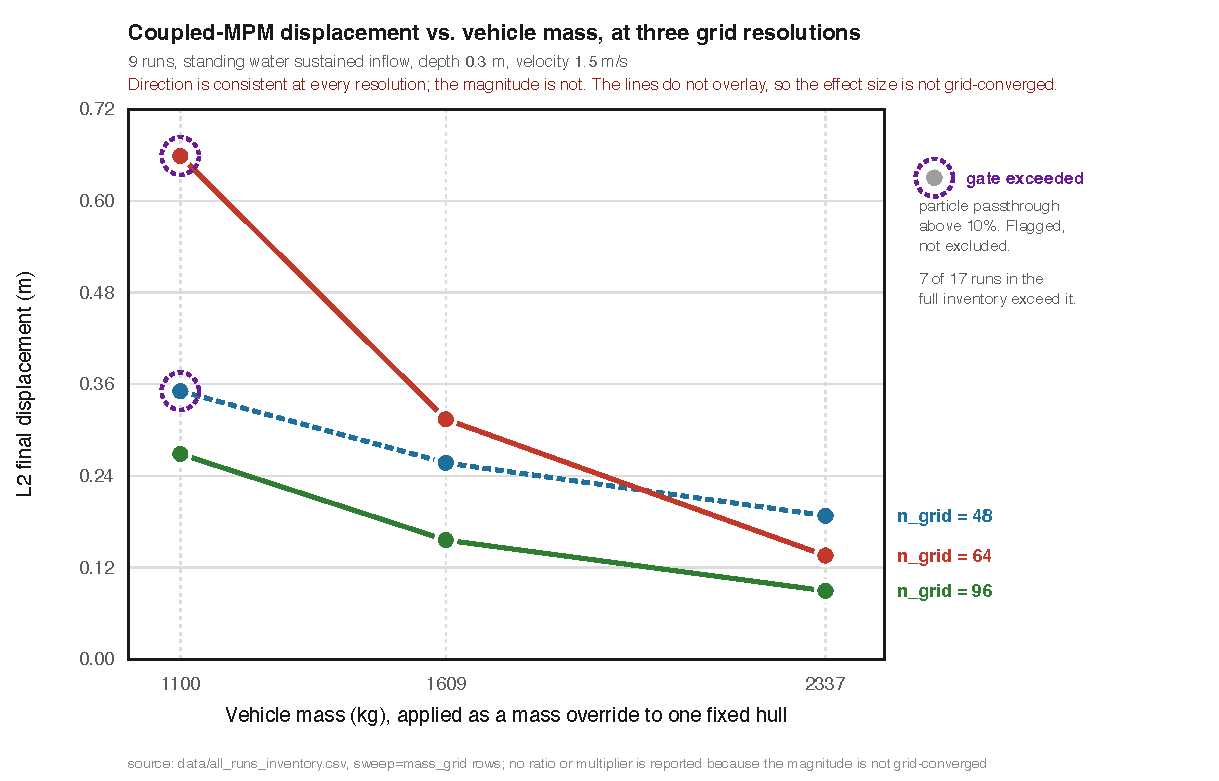
\includegraphics[width=\linewidth]{mass_grid_sweep_v2.pdf}
\caption{The direct visual for the 3\,$\times$\,3 mass-by-resolution block described in Section~\ref{subsec:sweep}: coupled-MPM final displacement versus vehicle mass at three grid resolutions, from the nine \texttt{sweep=mass\_grid} rows of \texttt{data/all\_runs\_inventory.csv}. One hull, three AR\&R mass overrides, fixed depth 0.30\,m and velocity 1.5\,m/s. Displacement decreases with mass at every resolution, but the curves do not collapse onto one another and the 48- and 64-cell curves cross, so the effect size is not grid-converged; no ratio or multiplier is reported for this reason. Ringed markers exceed the 10\% particle-passthrough limit and are flagged rather than excluded; 7 of the 17 runs in the full inventory exceed it.}
\label{fig:masssweep}
\end{figure}

Fig.~\ref{fig:l2render} shows a single frame from the 1100\,kg, \texttt{n\_grid}=64 member of that block.

\begin{figure}[t]
\centering
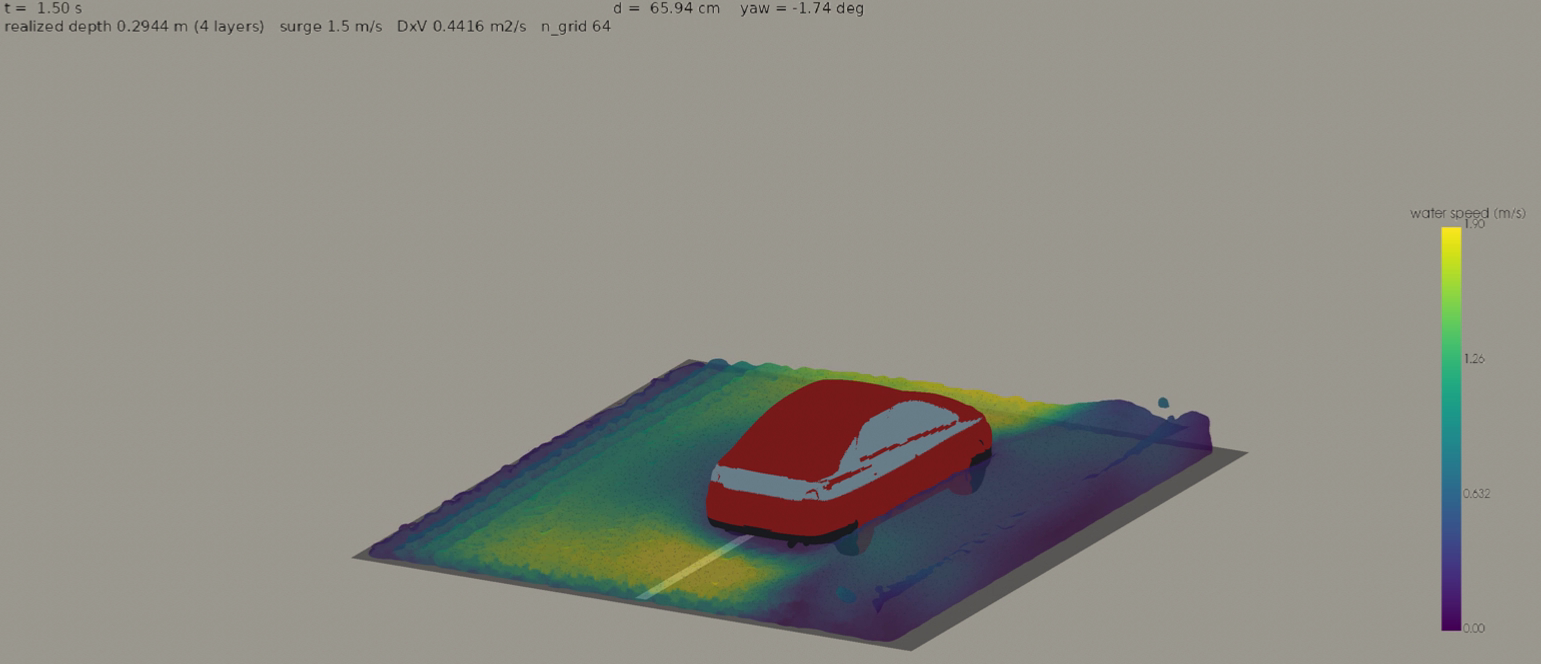
\includegraphics[width=\linewidth]{l2_render_g64_m1100_f0045.png}
\caption{One frame (45 of 90, $t = 1.50$\,s) from run \texttt{g64\_m1100} of the same \texttt{data/all\_runs\_inventory.csv} inventory: the watertight Yaris hull carried at 1100\,kg (AR\&R small passenger), \texttt{n\_grid}=64, requested depth 0.30\,m (realized 0.2944\,m, four water layers), and inflow velocity 1.5\,m/s, giving $D \times V = 0.4416$\,m\textsuperscript{2}/s. This is coupled-MPM solver output, not a Gaussian-splat reconstruction: the vehicle is the crash-validated finite-element hull carried as a rigid body, and the water surface is an isosurface reconstructed from the run's own MPM particles, coloured by water speed. The vehicle is drawn as the full watertight mesh posed by the rigid-body transform, while the physics ran on the 8{,}905 material points filling that hull. It is included to make the coupled simulation legible as a physical scene, not as a validated result. This run is one of the 7 of 17 that exceed the 10\% particle-passthrough gate, at 10.7\%, and the frame is mid-run, so the displacement printed in the frame is not the run's final reported value.}
\label{fig:l2render}
\end{figure}

% =================================================================
% V. CONCLUSIONS
% =================================================================
\section{Conclusions}
\label{sec:conclusions}

The synthetic-geometry pilot demonstrates, as a proof of concept, that a scalar depth-velocity hazard measure can disagree substantially with a coupled physical simulation, and that the disagreement is structural rather than a calibration artifact: no choice of coupling friction closes the gap at the divergence points identified in Section~\ref{sec:results}. This supports treating abstraction selection as query-dependent rather than assuming any single fixed-fidelity model is correct everywhere in the operating envelope.

We scope that conclusion deliberately. It is a pilot-study result on synthetic geometry, not a claim about the real reconstructed scene: the Drain A splat is not yet trained, the real-scene sweep is not yet verified, and the vehicle representation carries the mesh and density limitations set out in Section~\ref{sec:approach}. What this work establishes is that the divergence exists and is structural in the regime tested, which is what motivates the orchestrator; establishing where the escalation boundary falls for a real scene requires the verified real-scene sweep that remains future work.

% =================================================================
% VI. FUTURE WORK
% =================================================================
\section{Future Work}
\label{sec:future}

We identified several concrete extensions, listed roughly in order of expected impact relative to effort.

\begin{itemize}
\item \textbf{Crash-validated vehicle geometry.} NHTSA/NCAC publishes free, government-funded, crash-validated finite-element vehicle models (e.g., a 2010 Toyota Yaris sedan \cite{ccsa2016yaris} and a 2007 Chevrolet Silverado pickup) with real validated mass distribution, available in LS-DYNA keyword format and convertible to a simulation-ready collision mesh. We took the first step here. The Yaris hull in Section~\ref{sec:approach}-C is one of these models, and every AR\&R-linked result in this paper runs on it. What remains is the second step: using a different published model for each class, so the three classes differ in geometry and not only in mass.
\item \textbf{Physical-viability audit dashboard.} A direct instantiation of PVWM's ``physically viable'' criterion: automated checks for mass conservation, momentum conservation, MPM Jacobian/volume-ratio bounds, zero-penetration contact, and energy monotonicity, applied to every run rather than asserted informally.
\item \textbf{Failure-mode classification with violation magnitude.} An explicit failure-mode hierarchy (stuck, slide, topple, float) reported with the magnitude by which a run crosses each threshold, rather than a binary verdict.
\item \textbf{Graph Network Simulator (GNS) surrogate.} A lightweight GNS trained on the completed simulation sweep as a fast surrogate for untested (depth, velocity, vehicle-class) combinations, connecting the L0/L1/L2 ladder to a learned, still physically-grounded fourth level.
\item \textbf{A second independently-sourced real scene.} The Flooded Road Environments Dataset (FRED) captures on-road water hazards multi-modally, with camera, 64-beam LiDAR, and IMU/RTK-GNSS data from five locations recorded both during and after flooding, released with semantic labels in a KITTI-style format \cite{fred2026}. It is the natural second scene source for this pipeline: independent of our own capture, already labelled for water-hazard segmentation, and usable without a further field campaign.
\item \textbf{DesignSafe-CI dataset publication.} Publish the validated real-scene dataset and simulation outputs with a DOI once the real-scene sweep is verified, rather than publishing the synthetic pilot data.
\end{itemize}

% =================================================================
% ACKNOWLEDGMENT
% =================================================================
\section*{Acknowledgment}
This work was supported by the National Science Foundation under NSF REU Site: Cyberinfrastructure Research for Societal Advancement (SCIPE-AI), Award \#2447887, hosted at the Texas Advanced Computing Center (TACC), The University of Texas at Austin. The author thanks faculty mentor Dr.\ Krishna Kumar and research mentors Hassan Iqbal, Cheng-Hsi Hsiao, and Cristian Moran for their guidance throughout this project, and Rosalia Gomez for program coordination and support.

% =================================================================
% REFERENCES
% Uses BibTeX + IEEEtran.bst, matching the Zotero/Better-BibTeX
% auto-export pipeline. The official Overleaf gallery IEEE template
% does not ship IEEEtran.bst by default; upload the one provided
% alongside this file, or references will not resolve.
% =================================================================
\bibliographystyle{IEEEtran}
\bibliography{can_it_ford_references_IEEE}

\end{document}
